% Simple level diagram, resized and in a figure environment.
% Mark S. Everitt, 2009

\documentclass[10pt]{standalone}

% I only need the arrows for this one.
\usepackage{tikz}
\usetikzlibrary{arrows}

% New commands to keep things tidy.
\newcommand{\ket}[1]{$\left|#1\right\rangle$}
\newcommand{\Om}[1]{\small $\omega_{#1}$}
\newcommand{\De}[1]{$\Delta_{#1}$}
\newcommand{\Ga}[1]{$\Gamma_{#1}$}



\begin{document}


  \resizebox{7cm}{!}{
    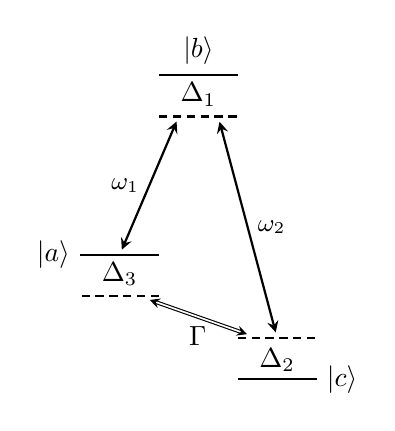
\begin{tikzpicture}[
      scale=0.5,
      level/.style={thick},
      virtual/.style={thick,densely dashed},
      trans/.style={thick,<->,shorten >=2pt,shorten <=2pt,>=stealth},
      classical/.style={thin,double,<->,shorten >=4pt,shorten <=4pt,>=stealth}
    ]
    % Draw the energy levels.
    \draw[level] (2cm,-2em) -- (0cm,-2em) node[left] {\ket{a}};
    \draw[level] (2cm,11em) -- (4cm,11em) node[midway,above] {\ket{b}};
    \draw[level] (4cm,-11em) -- (6cm,-11em) node[right] {\ket{c}};
    % Draw the virtual levels.
    \draw[virtual] (2cm,8em) -- (4cm,8em) node[midway,above] {\De{1}};
    \draw[virtual] (4cm,-8em) -- (6cm,-8em) node[midway,below] {\De{2}};
    \draw[virtual] (2cm,-5em) -- (0cm,-5em) node[midway,above] {\De{3}};
    % Draw the transitions.
    \draw[trans] (1cm,-2em) -- (2.5cm,8em) node[midway,left] {\Om{1}};
    \draw[trans] (3.5cm,8em) -- (5cm,-8em) node[midway,right] {\Om{2}};
    \draw[classical] (4.5cm,-8em) -- (1.5cm,-5em) node[midway,below] {\Ga{}};
    \end{tikzpicture}
  }


\end{document} 
